\documentclass{journal}
\usepackage{graphicx}
\usepackage{epstopdf}
\usepackage{overpic}
\usepackage{color}
\usepackage{amsmath}
\usepackage{amsfonts}
\usepackage{amsthm}
\usepackage{svg}


\theoremstyle{definition}
\newtheorem{definition}{Definition}
\newtheorem{theorem}{Theorem}
\newtheorem{lemma}{Lemma}
\newtheorem{corollary}{Corollary}
\newtheorem*{remark}{Remark}

\begin{document}
\title{Fourier Analysis of Daily Drinking Data}
\maketitle
\section{Introduction}
Mathematics in Psychology

\section{Fourier Transform of Time Series Data}
Caveats and best practices. Keith's work.

\section{Population Level Analysis of Drinking Data}
\begin{figure}[h]
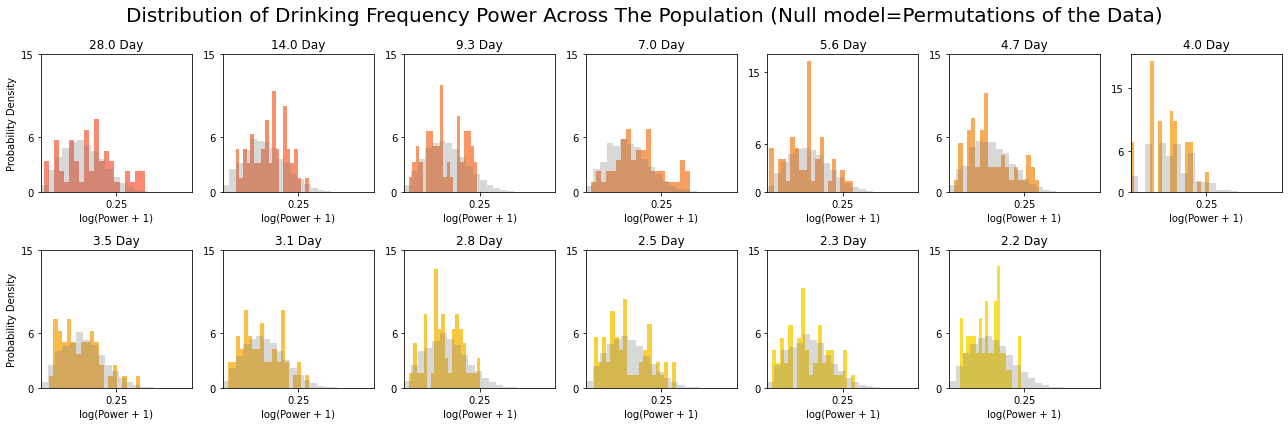
\includegraphics[width=\textwidth]{permutation_null_drinking_ft}
\end{figure}
\section{Individual Level Analysis of Drinking Data}

\section{Case Study in Better Data}

\end{document}
